\titleformat {\chapter} {\normalfont\huge\bfseries\color{black}}   {\thechapter}{10pt}{\huge} 
\chapter {Design View Point}

\section{Context View Point}

\subsection{Use Case Diagram}

\subsubsection{Use Case 1}
\vspace*{1\baselineskip}
\begin{figure}[htbp]
	\begin{center}
		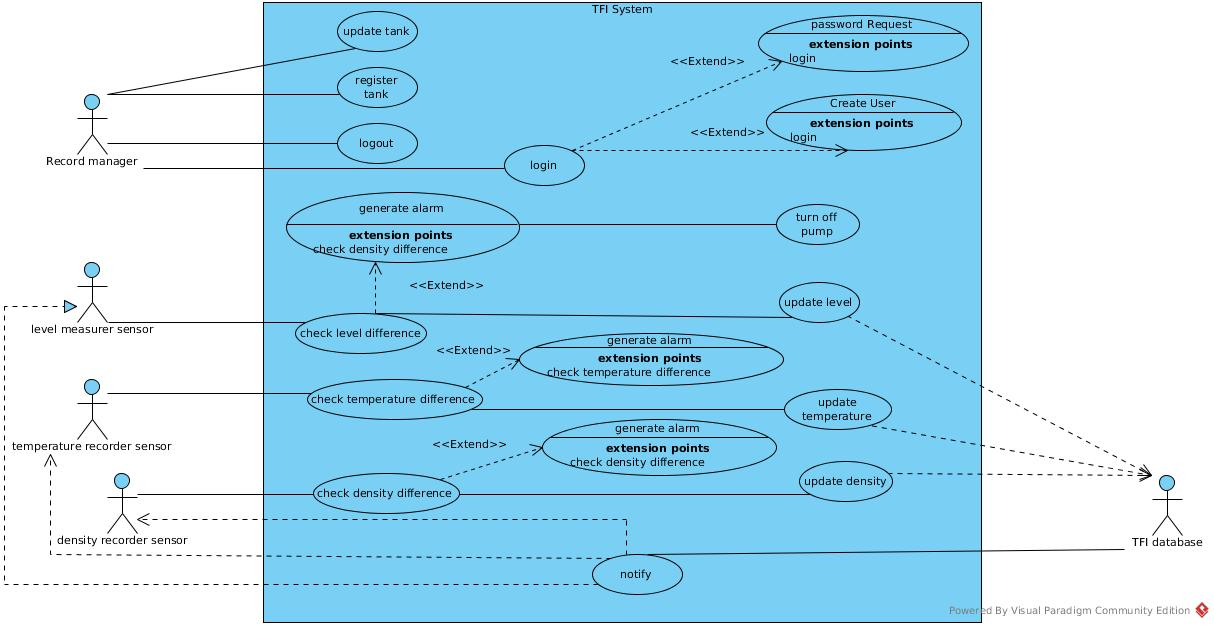
\includegraphics[width=\linewidth]{./images/UC01.jpg}
		\caption{1st Use case diagram for Tank Farm Inventory System.}
		\label{fig:UC01.jpg}
	\end{center}
\end{figure}


 \subsection{Description}
 \subsubsection{Record Manager :}
 
 \begin{center}
 \vspace*{1\baselineskip}	
 \begin{tabular}{|l|p{10cm}|}
 \hline
 Use Case ID: & UC001 \\
 \hline
 Use Case Name: & Update tank \\
 \hline
 Description: & This use case provides the functionality of updating Tank in the system \\
 \hline
 Primary Actor: & TFI Record Manager \\
 \hline
 Preconditions: & 1.The tank must have already been verified by the staff\\ 
			    & 2.The user should already be logged in the system \\
\hline
 Post Conditions: & The tank data should be stored in the dataset\\
\hline
\multicolumn{2}{|l|}{Main Scenario :} \\
\hline
\multicolumn{2}{|l|}{1.The user selects add tank option.} \\
\multicolumn{2}{|l|}{2.The user fills the tank information based on the physical(hard copy)data } \\
\multicolumn{2}{|l|}{3.The user selects to save the tank in the system} \\
\multicolumn{2}{|l|}{4.System shows the successful update of the tank data} \\
\hline
\multicolumn{2}{|l|}{Alternate Scenario :} \\
\hline
\multicolumn{2}{|l|}{TBD} \\
\hline	
\end{tabular}

\end{center}
		
			\begin{center}		
			\vspace*{1\baselineskip}	
			\begin{tabular}{|l|p{10cm}|}
				\hline
				Use Case ID: & UC002 \\
				\hline
				Use Case Name: & Register tank \\
				\hline
				Description: & This use case provides the functionality of registering Tank in the system \\
				\hline
				Primary Actor: & TFI Record manager \\
				\hline
				Preconditions: & 1.The tank must have already been verified by the staff\\ 
				& 2.The user should already be logged in the system \\
				\hline
				Post Conditions: & The tank data should be stored in the dataset\\
				\hline
				\multicolumn{2}{|l|}{Main Scenario :} \\
				\hline
				\multicolumn{2}{|l|}{1.The user selects add tank option.} \\
				\multicolumn{2}{|l|}{2.The user fills the tank information based on the physical(hard copy)data } \\
				\multicolumn{2}{|l|}{3.The user selects to save the tank in the system} \\
				\multicolumn{2}{|l|}{4.System shows the successful update of the tank data} \\
				\hline
				\multicolumn{2}{|l|}{Alternate Scenario :} \\
				\hline
				\multicolumn{2}{|l|}{Start after step 2 in the main scenario:} \\
				\multicolumn{2}{|l|}{1.The entered tank is already registered in the system} \\
				\multicolumn{2}{|l|}{2.The system shows an error message "Already Registered Tank"} \\
				\multicolumn{2}{|l|}{3.It returns to step 1 of the main scenario} \\
				\hline
			\end{tabular}
			\end{center}	
			
			
	\subsubsection{Level Measurer Sensor :}
			\begin{center}
			\vspace*{1\baselineskip}	
			\begin{tabular}{|l|p{10cm}|}
				\hline
				Use Case ID: & UC003 \\
				\hline
				Use Case Name: & Check level difference \\
				\hline
				Description: & This use case provides the functionality of checking the level difference \\
				\hline
				Primary Actor: & Level measure sensor \\
				\hline
				Preconditions: & 1.The leveler must have already been verified by the staff\\ 
				& 2.The user should already be logged in the system \\
				\hline
				Post Conditions: & The level data should be stored in the dataset\\
				\hline
				\multicolumn{2}{|l|}{Main Scenario :} \\
				\hline
				\multicolumn{2}{|l|}{1.The user checks level difference.} \\
				\multicolumn{2}{|l|}{2.The user update level} \\
				\multicolumn{2}{|l|}{3.The user check generate alarm and decide state of pump} \\
				\multicolumn{2}{|l|}{4.User update level into database.} \\
				\hline
				\multicolumn{2}{|l|}{Alternate Scenario :} \\
				\hline
				\multicolumn{2}{|l|}{Start after step 2 in the main scenario:} \\
				\multicolumn{2}{|l|}{1.User will get notification from TFI database.} \\
				\hline
			\end{tabular}
			\end{center}
			
			
			
		\subsubsection{Temperature Measurer sensor :}
				\begin{center}
				\vspace*{1\baselineskip}	
				\begin{tabular}{|l|p{10cm}|}
					\hline
					Use Case ID: & UC004 \\
					\hline
					Use Case Name: & Check temperature difference \\
					\hline
					Description: & This use case provides the functionality of checking the temperature difference \\
					\hline
					Primary Actor: & Temperature recorder sensor \\
					\hline
					Preconditions: & 1.The temperature must have already been verified by the staff\\ 
					& 2.The user should already be logged in the system \\
					\hline
					Post Conditions: & The temperature data should be stored in the dataset\\
					\hline
					\multicolumn{2}{|l|}{Main Scenario :} \\
					\hline
					\multicolumn{2}{|l|}{1.The user checks temperature difference.} \\
					\multicolumn{2}{|l|}{2.The user update temperature into database} \\
					\hline
					\multicolumn{2}{|l|}{Alternate Scenario :} \\
					\hline
					\multicolumn{2}{|l|}{User will get notification from TFI Database} \\
					\hline
				\end{tabular}
				\end{center}
				
				
				
		\newpage
		\subsubsection{Density Measurer sensor :}
		\begin{center}
			\vspace*{1\baselineskip}	
			\begin{tabular}{|l|p{10cm}|}
				\hline
				Use Case ID: & UC005 \\
				\hline
				Use Case Name: & Check density difference \\
				\hline
				Description: & This use case provides the functionality of checking the density difference \\
				\hline
				Primary Actor: & Density recorder sensor \\
				\hline
				Preconditions: & 1.The density must have already been verified by the staff\\ 
				& 2.The user should already be logged in the system \\
				\hline
				Post Conditions: & The density data should be stored in the dataset\\
				\hline
				\multicolumn{2}{|l|}{Main Scenario :} \\
				\hline
				\multicolumn{2}{|l|}{1.The user checks density difference.} \\
				\multicolumn{2}{|l|}{2.The user update density into database} \\
				\hline
				\multicolumn{2}{|l|}{Alternate Scenario :} \\
				\hline
				\multicolumn{2}{|l|}{User will get notification from TFI Database} \\
				\hline
			\end{tabular}
		\end{center}
				
				
		
\clearpage
\subsubsection{Use Case 2}
\vspace*{1\baselineskip}
\begin{figure}[htbp]
	\begin{center}
		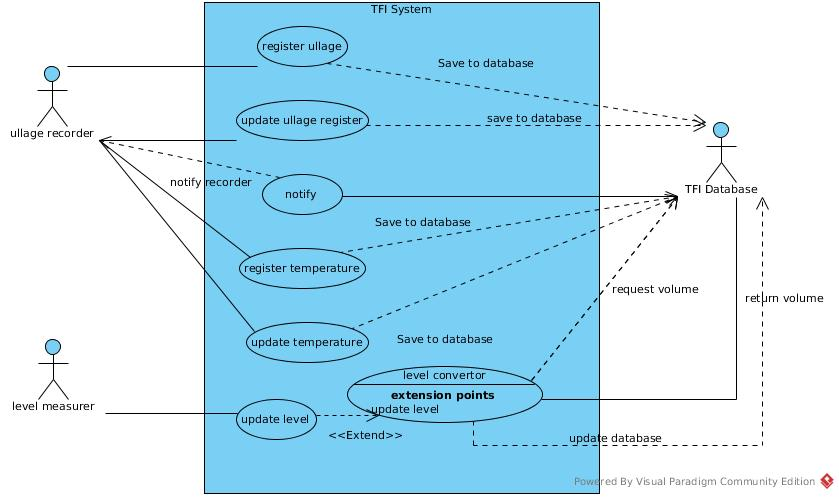
\includegraphics[width=\linewidth]{./images/UC003.jpeg}
		\caption{2nd Use case diagram for Tank Farm Inventory System.}
		\label{fig:UC003.jpeg}
	\end{center}
\end{figure}

\nopagebreak

	\subsection{Description}
	\subsubsection{Ullage Recorder :}
	\begin{center}
	\vspace*{1\baselineskip}	
	\begin{tabular}{|l|p{10cm}|}
		\hline
		Use Case ID: & UC006 \\
		\hline
		Use Case Name: & Register ullage \\
		\hline
		Description: & This use case provides the functionality of registering ullage \\
		\hline
		Primary Actor: & Ullage recorder \\
		\hline
		Preconditions: & 1.The ullage must have already been verified by the staff\\ 
		& 2.The user should already be logged in the system \\
		\hline
		Post Conditions: & The ullage data should be stored in the dataset\\
		\hline
		\multicolumn{2}{|l|}{Main Scenario :} \\
		\hline
		\multicolumn{2}{|l|}{1.The user registers ullage.} \\
		\multicolumn{2}{|l|}{2.The data will saved to database} \\
		\hline
		\multicolumn{2}{|l|}{Alternate Scenario :} \\
		\hline
		\multicolumn{2}{|l|}{User will get notification from TFI Database} \\
		\hline
	\end{tabular}
\end{center}
	
		\begin{center}	
		\vspace*{1\baselineskip}	
		\begin{tabular}{|l|p{10cm}|}
			\hline
			Use Case ID: & UC007 \\
			\hline
			Use Case Name: & Update ullage register \\
			\hline
			Description: & This use case provides the functionality of registering ullage \\
			\hline
			Primary Actor: & Ullage sensor \\
			\hline
			Preconditions: & 1.The Ullage must have already been verified by the staff\\ 
			& 2.The user should already be logged in the system \\
			\hline
			Post Conditions: & The ullage data should be stored in the dataset\\
			\hline
			\multicolumn{2}{|l|}{Main Scenario :} \\
			\hline
			\multicolumn{2}{|l|}{1.The user registers ullage.} \\
			\multicolumn{2}{|l|}{2.The data will be saved to database} \\
			\hline
			\multicolumn{2}{|l|}{Alternate Scenario :} \\
			\hline
			\multicolumn{2}{|l|}{User will get notification from TFI Database} \\
			\hline
		\end{tabular}
	\end{center}
	
	
	\begin{center}
	\vspace*{1\baselineskip}	
	\begin{tabular}{|l|p{10cm}|}
		\hline
		Use Case ID: & UC008 \\
		\hline
		Use Case Name: & Register temperature \\
		\hline
		Description: & This usecase provides the functionality of register temperature \\
		\hline
		Primary Actor: & Ullage recorder \\
		\hline
		Preconditions: & 1.The temperature must have already been verified by the staff\\ 
		& 2.The user should already be logged in the system \\
		\hline
		Post Conditions: & The temperature data should be stored in the dataset\\
		\hline
		\multicolumn{2}{|l|}{Main Scenario :} \\
		\hline
		\multicolumn{2}{|l|}{1.The user registers temperature} \\
		\multicolumn{2}{|l|}{2.The data will be saved to database } \\
		\multicolumn{2}{|l|}{Alternate Scenario :} \\
		\hline
		\multicolumn{2}{|l|}{TBD} \\
		\hline
	\end{tabular}
\end{center}

	\begin{center}
	\vspace*{1\baselineskip}	
	\begin{tabular}{|l|p{10cm}|}
		\hline
		Use Case ID: & UC009 \\
		\hline
		Use Case Name: & Update temperature \\
		\hline
		Description: & This usecase provides the functionality of update temperature \\
		\hline
		Primary Actor: & Ullage recorder \\
		\hline
		Preconditions: & 1.The temperature must have already been verified by the staff\\ 
		& 2.The user should already be logged in the system \\
		\hline
		Post Conditions: & The temperature data should be stored in the dataset\\
		\hline
		\multicolumn{2}{|l|}{Main Scenario :} \\
		\hline
		\multicolumn{2}{|l|}{1.The user updates temperature.} \\
		\multicolumn{2}{|l|}{2.The data will be saved to database } \\
		\hline
		\multicolumn{2}{|l|}{Alternate Scenario :} \\
		\hline
		\multicolumn{2}{|l|}{1.The updated temperature will be saved into database} \\
		\hline
	\end{tabular}
	\end{center}
	
	
    \subsubsection{Level Measurer :}	
	\begin{center}
	\vspace*{1\baselineskip}	
	\begin{tabular}{|l|p{10cm}|}
		\hline
		Use Case ID: & UC0010 \\
		\hline
		Use Case Name: & Update Level \\
		\hline
		Description: & This usecase provides the functionality of update level \\
		\hline
		Primary Actor: & Level measurer \\
		\hline
		Preconditions: & 1.The level  must have already been verified by the staff\\ 
		& 2.The user should already be logged in the system \\
		\hline
		Post Conditions: & The level data should be stored in the dataset\\
		\hline
		\multicolumn{2}{|l|}{Main Scenario :} \\
		\hline
		\multicolumn{2}{|l|}{1.The user updates level.} \\
		\multicolumn{2}{|l|}{2.The data will be saved to database } \\
		\hline
		\multicolumn{2}{|l|}{Alternate Scenario :} \\
		\hline
		\multicolumn{2}{|l|}{1.The updated temperature will be converted for volume in the database} \\
		\multicolumn{2}{|l|}{2.Database will be updated with volume once converting done.} \\
		\hline
	\end{tabular}
	\end{center}
	
	
	
\newpage	
\subsubsection{Use Case 3}
\vspace*{1\baselineskip}
\begin{figure}[htbp]
	\begin{center}
		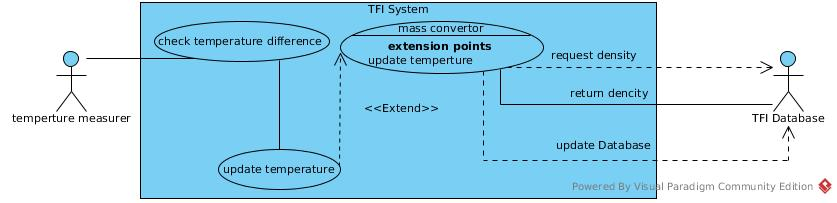
\includegraphics[width=1.00\linewidth]{./images/UC03.jpg}
		\caption{3rd Use case diagram for Tank Farm Inventory System.}
		\label{fig:UC03.jpg}
	\end{center}
\end{figure}

\nopagebreak

\subsection{Description}
\subsubsection{Temperature Measurer :}
\begin{center}
\vspace*{1\baselineskip}	
\begin{tabular}{|l|p{10cm}|}
	\hline
	Use Case ID: & UC0011 \\
	\hline
	Use Case Name: & Update temperature \\
	\hline
	Description: & This usecase provides the functionality of update temperature \\
	\hline
	Primary Actor: & Temperature measurer \\
	\hline
	Preconditions: & 1.The temperature must have already been verified by the staff\\ 
	& 2.The user should already be logged in the system \\
	\hline
	Post Conditions: & The temperature data should be stored in the dataset\\
	\hline
	\multicolumn{2}{|l|}{Main Scenario :} \\
	\hline
	\multicolumn{2}{|l|}{1.The user updates temperature.} \\
	\multicolumn{2}{|l|}{2.The data will be saved to database } \\
	\hline
	\multicolumn{2}{|l|}{Alternate Scenario :} \\
	\hline
	\multicolumn{2}{|l|}{1.The updated temperature will be converted for volume in the database} \\
	\multicolumn{2}{|l|}{2.Database will be updated with volume once converting done.} \\
	\multicolumn{2}{|l|}{3.Database will request for density for the mass converter.} \\
	\hline
\end{tabular}
\end{center}			


\newpage
\subsubsection{Use Case 4}
\vspace*{1\baselineskip}
\begin{figure}[htbp]
	\begin{center}
		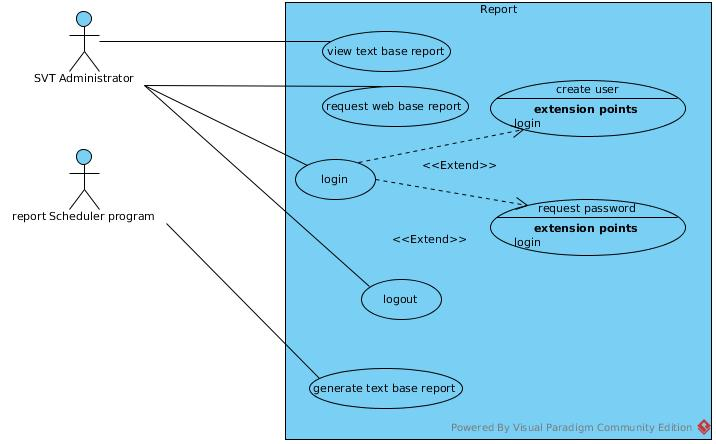
\includegraphics[width=1.00\linewidth]{./images/UC004.jpeg}
		\caption{4th Use case diagram for Tank Farm Inventory System.}
		\label{fig:UC004.jpeg}
	\end{center}
\end{figure}

\nopagebreak

\subsection{Description}
\subsubsection{SVT Administrator :}
\begin{center}
\vspace*{1\baselineskip}	
\begin{tabular}{|l|p{10cm}|}
	\hline
	Use Case ID: & UC0012 \\
	\hline
	Use Case Name: & View text based report \\
	\hline
	Description: & This usecase provides the functionality of viewing text based report \\
	\hline
	Primary Actor: & TFI Administrator \\
	\hline
	Preconditions: & 1.The report is generated automatically\\ 
	& 2.The user should already be logged in the system \\
	\hline
	Post Conditions: & \\
	\hline
	\multicolumn{2}{|l|}{Main Scenario :} \\
	\hline
	\multicolumn{2}{|l|}{1.The user view text based report.} \\
	\hline
	\multicolumn{2}{|l|}{Alternate Scenario :} \\
	\hline
	\multicolumn{2}{|l|}{TBD} \\
	\hline
\end{tabular}
\end{center}

\begin{center}
\vspace*{1\baselineskip}	
\begin{tabular}{|l|p{10cm}|}
	\hline
	Use Case ID: & UC0013 \\
	\hline
	Use Case Name: & Request web based report \\
	\hline
	Description: & This usecase provides the functionality of request for web based report. \\
	\hline
	Primary Actor: & TFI Administrator \\
	\hline
	Preconditions: & 1.The report is generated automatically\\ 
	& 2.The user should already be logged in the system \\
	\hline
	Post Conditions: & \\
	\hline
	\multicolumn{2}{|l|}{Main Scenario :} \\
	\hline
	\multicolumn{2}{|l|}{1.The user request web based report.} \\
	\hline
	\multicolumn{2}{|l|}{Alternate Scenario :} \\
	\hline
	\multicolumn{2}{|l|}{TBD} \\
	\hline
\end{tabular}
\end{center}

	\subsubsection{Report Scheduler Program :}
	\begin{center}
	\vspace*{1\baselineskip}	
	\begin{tabular}{|l|p{10cm}|}
		\hline
		Use Case ID: & UC0014 \\
		\hline
		Use Case Name: & Generate text base report \\
		\hline
		Description: & This use case provides the functionality of generating text based report \\
		\hline
		Primary Actor: & Report scheduler program \\
		\hline
		Preconditions: & 1.The request is received\\ 
		& 2.The user should already be logged in the system \\
		\hline
		Post Conditions: & Generate report based on specific details that obtained from users\\
		\hline
		\multicolumn{2}{|l|}{Main Scenario :} \\
		\hline
		\multicolumn{2}{|l|}{1.The program generates web based report.} \\
		\hline
		\multicolumn{2}{|l|}{Alternate Scenario :} \\
		\hline
		\multicolumn{2}{|l|}{TBD} \\
		\hline
	\end{tabular}
	\end{center}


\newpage
\subsubsection{Use Case 5}
\vspace*{0.5\baselineskip}
\begin{figure}[htbp]
	\begin{center}
		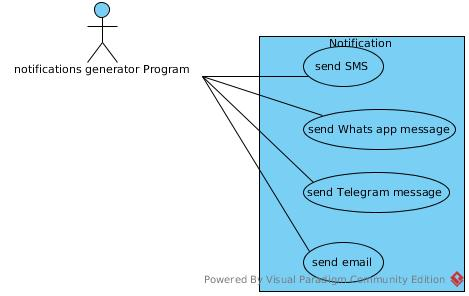
\includegraphics[width=0.85\linewidth]{./images/UC005.jpeg}
		\caption{5th Use case diagram for Tank Farm Inventory System.}
		\label{fig:UC005.jpeg}
	\end{center}
\end{figure}



\subsection{Description}
\subsubsection{Notification Generator Program :}
\begin{center}
\vspace*{1\baselineskip}	
\begin{tabular}{|l|p{10cm}|}
	\hline
	Use Case ID: & UC0015 \\
	\hline
	Use Case Name: & Notification \\
	\hline
	Description: & This use case provides the functionality of notifying user\\
	\hline
	Primary Actor: & Notification generator program \\
	\hline
	Preconditions: & 1.The operation is transacted\\ 
	& 2.The user should already be logged in the system \\
	\hline
	Post Conditions: & Generate into different form such as SMS,Whatsapp,Telegram and email\\
	\hline
	\multicolumn{2}{|l|}{Main Scenario :} \\
	\hline
	\multicolumn{2}{|l|}{1.The program generates notification.} \\
	\hline
	\multicolumn{2}{|l|}{Alternate Scenario :} \\
	\hline
	\multicolumn{2}{|l|}{TBD} \\
	\hline
\end{tabular}
\end{center}









